\chapter{Memorias}
\label{cap:memorias}

La memoria es un acto en el presente. En tal acto, tanto la imaginación como las experiencias, las competencias, las emociones, los sentimientos y los sesgos personales no pueden no influir. Las expectativas personales y sociales también pesan en el presente acto de recordar. \emph{Recordar} es volver a pasar por el corazón, \emph{recordar} volver a sonar. Con esto en mente, con la conciencia de que recordar es un acto creativo, intento traer a mi memoria tanto la primer reunión con las autoridades universitarias como la reunión entre «Pajarito», Juan Martín y yo.


\section{El canto y las palabras de un hijo}
\label{sec:palabra-canto}

\begin{figure}[H]
\centering
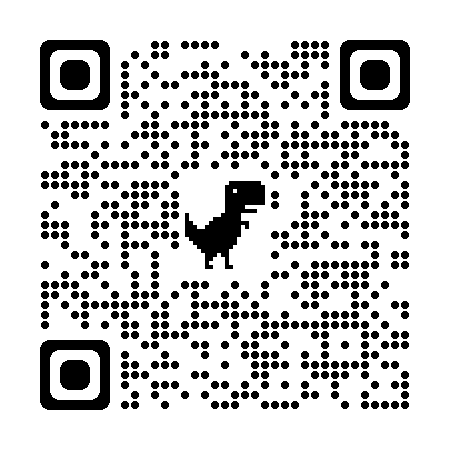
\includegraphics[width=0.3\textwidth]{img/qrcode-himno-memoria}
\caption{El canto y las palabras de \textsc{Juan Martín Leguizamón}.}
\label{fig:canto-palabras}
\end{figure}


En diciembre de 2022 me contacta \textsc{Marcelo «Pajarito» Sutti}\footnote{\textsc{Marcelo Sutti} es destacado poeta y músico salteño.}, quien me informa que \textsc{Juan Martín Leguizamón}\footnote{\textsc{Juan Martín Leguizamón}, hijo de Gustavo, es antropólogo y presidente de la Fundación Legado Cultural Cuchi Leguizamón.} le refiere tener viva en su memoria una melodía que recuerda como el \emph{Himno a la UNSa}. Enteradas las autoridades de la Universidad del relato de Juan Martín ---y mediado por Sutti quien me señala como un hombre idóneo para realizar un peritaje sobre la melod´ia en memoria del hijo del «Cuchi»---, organizan una reunión en la que acordamos trabajar sobre el fragmento recordado y su posible relación con los modos de componer del legendario músico saleño. La posibilidad de establecer un grado de compatibilidad entre la melodía a estudiar y las melodías de Gustavo Leguizamón existe porque existen técnicas de análisis que pueden develar estructuras análogas en diversas piezas de un mismo autor. El \emph{análisis schenkeriano} en el particular caso me pareció una herramienta adecuada por ser capaz de mostrar estructuras intermedias y de superficie propias de un autor es específico, y es la que propuse en esa reunión utilizar en la pericia.

No recuerdo si primero fue la reunión con las autoridades universitarias, o si antes fue la reunión con Sutti y Leguizamón (h). No importa. Sí importa que fue una tardecita de verano con un cielo tapado de poderosas y negras nubes. El momento central de esa amena charla no es necesario recordarlo: el registro electrónico nos exime del acto creativo de recordar, y él es accesible con el código QR de la Figura~\ref{fig:canto-palabras}.
